% Build instructions for the 100 mm kaleidoscope prototype.
\documentclass[letterpaper,11pt]{article}
\usepackage[letterpaper,top=20mm,bottom=20mm,left=22mm,right=22mm]{geometry}
\usepackage[T1]{fontenc}
\usepackage{parskip}
\usepackage{enumitem}
\usepackage{booktabs}
\usepackage{tikz}
\usepackage{xcolor}
\usetikzlibrary{arrows.meta}

\definecolor{reg}{gray}{0.45}
\definecolor{mir}{rgb}{0.15,0.40,0.65}

\setlist[enumerate]{itemsep=2pt,topsep=4pt}
\setlist[itemize]{itemsep=2pt,topsep=4pt}

\newcommand{\head}[1]{\vspace{3mm}\textbf{\large #1}\vspace{1mm}\hrule\vspace{2mm}}

% ── one rail's cross-section at the narrow end, in mm about the tube axis ──
\newcommand{\railpath}{%
  (-13.700,-9.1325) -- (15.818,-9.1325) -- (14.759,-7.2985) --
  (15.538,-6.8485) -- (15.138,-6.1557) -- (16.177,-5.5557) --
  (16.577,-6.2485) -- (17.357,-5.7985) -- (21.014,-12.1325) --
  (-13.700,-12.1325) -- (-13.700,-11.3825) -- (-12.750,-11.3825) --
  (-12.750,-9.8825) -- (-13.700,-9.8825) -- cycle}
% mirror spans from the split face (overlap edge, flush at -13.70) to the
% ideal vertex at +12.70, where its leading edge stops on the neighbour.
\newcommand{\mirrorpath}{(-13.70,-7.33249) rectangle (12.7,-8.93249)}

\begin{document}

\begin{center}
  {\LARGE\bfseries Tapered kaleidoscope --- 100\,mm prototype}\\[2mm]
  {\large Cutting and assembly}
\end{center}

\vspace{2mm}

Three identical printed rails, each carrying one flat trapezoidal mirror, lapped together
at the corners into a truncated triangular pyramid. Because the three mirror planes
converge on a common apex 100\,mm beyond the narrow end, the images tile a \emph{sphere}
rather than the flat honeycomb an untapered scope produces. You look in the wide end; the
glass chips go at the narrow end.

\begin{center}
\begin{tabular}{@{}ll@{}}
\toprule
Mirror-face triangle & 25.40\,mm at the narrow end, 50.80\,mm at the wide end \\
Length along the axis & 100\,mm \\
Taper half-angle & 4.1936$^\circ$ \\
Corner dihedral & 60.529286$^\circ$ \emph{(not 60 --- the excess is the whole effect)} \\
Image & a sphere subtending 60$^\circ$, about 453 facets \\
Optical face & 25.40\,mm at the narrow end, 50.80\,mm at the wide end \\
Mirror blank & trapezoid, parallel edges 26.40 and 51.80, height 100.27, legs 101.07\,mm \\
 & (the face plus 1.00\,mm of overlap allowance --- see \S4) \\
\bottomrule
\end{tabular}
\end{center}

\head{1. Print the rails}

Three copies of the same part --- there is no left or right hand. Laid flat the part is
\textbf{60.1 $\times$ 100.3\,mm and 6.54\,mm tall}, so all three fit on an MK3 bed at once
(190.3 $\times$ 100.3\,mm), and printing them together keeps all three under identical
conditions.

The model already sits with its outside face on the XY plane. Its steepest overhang is
29.5$^\circ$ --- the underside of the tongue --- against a 55$^\circ$ threshold, and the only
near-horizontal face is the groove ceiling, which is a 0.95\,mm bridge rather than an
overhang. \textbf{No supports, and none of this is marginal.}

\medskip

\textbf{PrusaSlicer, MK3 with PLA, 0.4\,mm nozzle.} Start from
\emph{0.15\,mm QUALITY @MK3} and change only these:

\begin{center}
\begin{tabular}{@{}lll@{}}
\toprule
\textbf{Setting} & \textbf{Value} & \textbf{Why} \\
\midrule
Ironing & On, \emph{topmost surface only} & the pocket floor is the mirror seat \\
Perimeters & 3 & makes the 3\,mm wall nearly solid \\
Elephant foot compensation & 0.2\,mm (verify) & split faces run down to the bed \\
Perimeter generator & Arachne (default) & handles the 1.2\,mm tongue \\
Layer height & 0.15\,mm & 44 layers; the part is all flat planes \\
Fill density & 15\,\% & fine as-is; perimeters do the work \\
Supports & None & 29.5$^\circ$ maximum overhang \\
Brim & None & 60 $\times$ 100\,mm flat footprint, no warp risk \\
Seam position & Rear or Aligned & cosmetic only, on the outside face \\
\bottomrule
\end{tabular}
\end{center}

\medskip

Only the first three are worth arguing about.

\textbf{Ironing} matters most. The pocket floor is a \emph{top} surface, and at 1.59\,mm your
mirror is thin enough to conform to whatever that floor does --- print texture becomes optical
texture. Ironing is what stops that. With rigid mirror stock it would not matter.

\textbf{Three perimeters} rather than two. At 0.45\,mm extrusion width that makes the 3\,mm
wall effectively solid. On a part this thin, perimeters do far more for stiffness and for
tongue-and-groove strength than infill does --- which is also why 15\,\% fill needs no change.

\textbf{Elephant foot compensation} is not cosmetic here. The split face and both mating faces
run right down to the bed, so first-layer squish-out directly prevents the corners closing.
0.2\,mm is the Prusa default; just confirm it has not been zeroed.

Dropping to 0.20\,mm layers (33 layers) is fine if you would rather iterate faster --- the
geometry is entirely flat planes and ironing works independently of layer height. STL export
quality is irrelevant for the same reason: the part has no curved surfaces at all, so even the
coarsest tessellation is exact.

\medskip

\textbf{Print a joint test coupon first.} All three rails are identical, so if the
tongue-and-groove clearance is wrong, all three are wrong together --- and at 0.15\,mm
clearance with a 0.4\,mm nozzle that fit is the likeliest thing to need adjusting, since a
1.2\,mm tongue is under three extrusions wide and the usual bias is tongues fat and grooves
narrow. Use PrusaSlicer's \emph{Cut} tool to take a 20\,mm slice off the model, keep one half,
add a second instance, print the pair. Ten minutes instead of two hours, and you learn whether
to open \texttt{tongueClearance} to 0.2 first.

Do not shortcut this by regenerating a 20\,mm part in Onshape --- that changes the taper
completely and gives you a different triangle. Cut the 100\,mm model.

\head{2. About the mirror stock}

The cheap ``unbreakable'' tiles are plastic, not glass, so ignore anything you read about
glass cutters and running pliers. Two honest warnings:

\begin{itemize}[leftmargin=*]
\item \textbf{They are sold for safety, not optics, and are usually noticeably wavy.}
      Flatness is the single most important optical property of a kaleidoscope mirror, so
      expect a soft, smeary image with visible distortion in the outer facets. Do not judge
      the design by what these produce --- judge the fit, the corners and the workflow.
\item \textbf{The panels are 1/16$''$}, so \texttt{mirrorThickness} is 1.5875\,mm and the
      pocket comes out at 1.7875\,mm. That leaves 0.2\,mm of headroom, and the error is
      one-sided: stock thinner than nominal is harmless, because the bond layer takes up the
      slack. Only stock more than 0.2\,mm \emph{over} nominal causes trouble, by holding the
      mirror faces proud so the corners interfere.
\end{itemize}

\head{3. Cutting the mirrors}

\textbf{Do not use the rotary cutters.} They are built to shear fabric against a mat, not
to score rigid plastic. The blades are thin and hardened and will chip on the first pass,
and they cost more than the tiles. (If the sheet turns out to be under about half a
millimetre and genuinely floppy, a rotary cutter will work --- test on a scrap corner.)
The utility knife and the sewing ruler are the right pair; the ruler's printed grid is
better for this than a plain straightedge.

\begin{enumerate}[leftmargin=*]
\item \textbf{Check the template.} Print \texttt{mirror-template.pdf} at 100\,\% ---
      \emph{Actual size}, not \emph{Fit to page} --- and verify both rulers on it with a
      real ruler. If they are off, every dimension is off.
\item \textbf{Coated side up.} These are rear-surface mirrors: clear plastic in front, the
      reflective coating on the back under a paint layer. Cut with the coated side facing
      you. The blade then enters through the coating while it is still fully supported by
      the plastic beneath, which gives a clean coating edge --- and the tear-out from the
      final pass lands on the clear face, where it does not matter. Cut the other way round
      and the last pass tears the coating back from the edge, which is the one defect this
      design cannot tolerate. Slip a sheet of paper under the clear face so the mat cannot
      mark it.
\item \textbf{Leave the protective film on} and mark on it. It prevents scratches and the
      blade tracks better.
\item \textbf{Transfer the marks.} Tape the template over the tile, prick through the
      centre of all twelve circled marks with a pin, lift the paper, and join the pricks
      with the straightedge. Marking through paper beats cutting through it --- a knife
      shreds paper and then wanders.
\item \textbf{Score.} Put the ruler on the side you are keeping, so a slip runs into the
      waste. Hold it down hard; more failures here come from the ruler creeping than from
      the knife wandering. Draw the knife along the line six to ten times with moderate,
      consistent pressure, same track each time, aiming to get about halfway through. Do
      not try to power through in one pass.
\item \textbf{Snap --- or don't.} Score up, overhang past a table edge, hold the tile flat,
      press down sharply and evenly. Thin plastic often \emph{bends instead of breaking};
      unlike glass it has no clean cleavage. If it flexes rather than snapping, stop and
      keep scoring until you are through. Slower, but far more reliable, and on 100\,mm
      pieces it is only a couple of minutes.
\item \textbf{Finish the two long edges.} Lay 400-grit flat on the table, hold the piece
      vertical, two or three light passes per edge. Keep it square --- do not round it
      over, and do not sand onto the reflective face.
\item \textbf{Check the coating.} Hold each long edge up to the light. The silver must run
      right to the edge; any dead band there prints as a dark web across every facet.
\end{enumerate}

\textbf{Only two of the four edges matter.} The slanted 101.07\,mm sides butt against the
neighbouring mirrors. The 26.40 and 51.80\,mm ends are hidden under the end caps and can be
rough. Cut on the line --- a scored edge removes essentially nothing --- and if a blank
drifts a few tenths wide, leave it; the overlap allowance absorbs it (\S4).

\head{4. Where the mirror sits}

\begin{center}
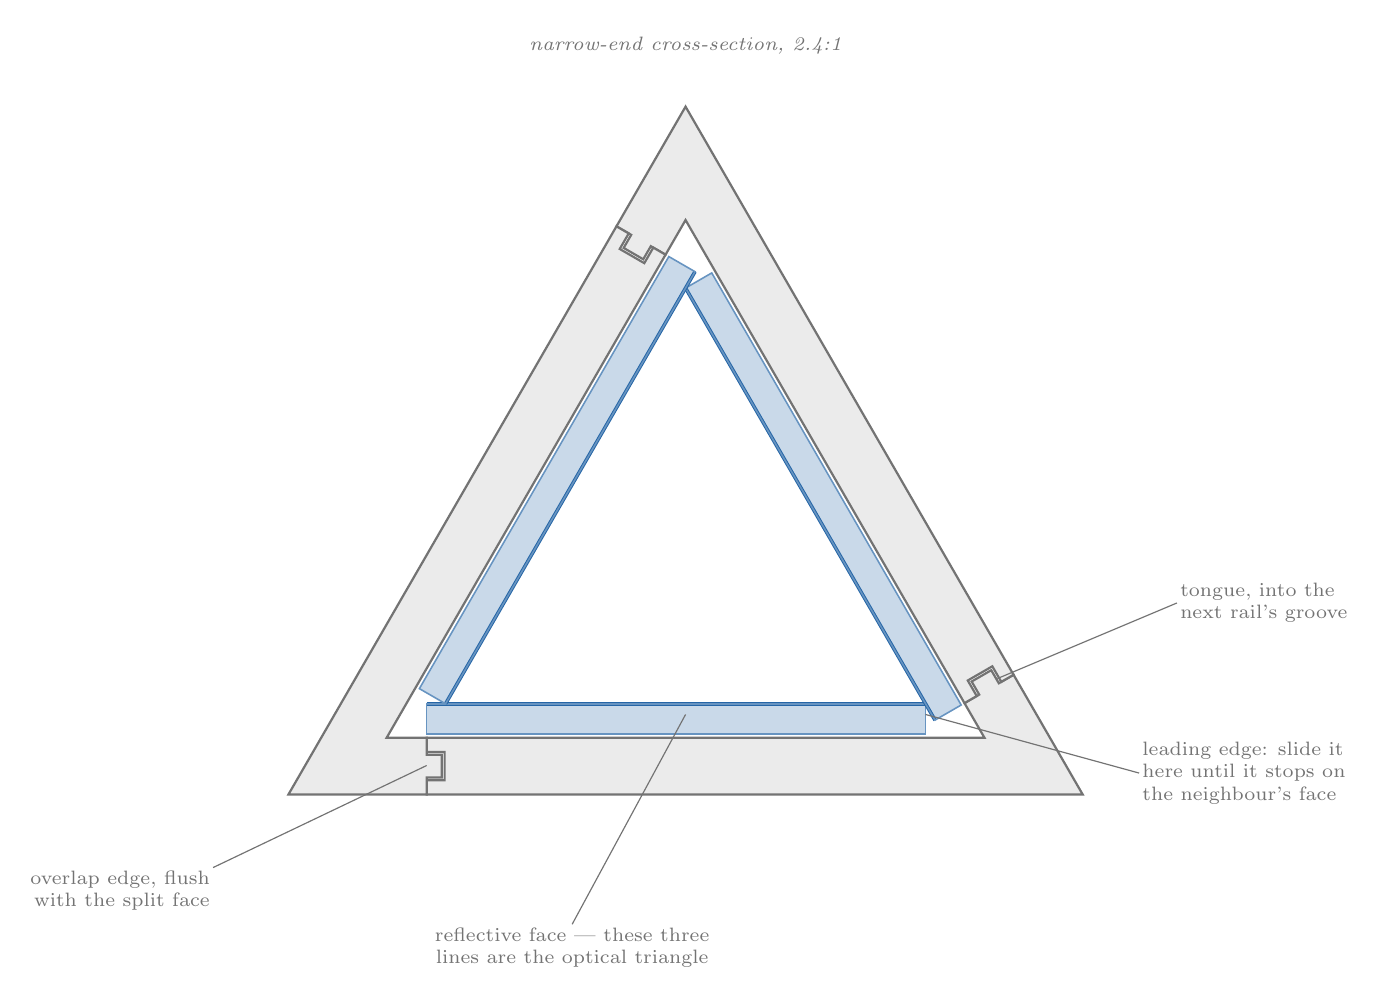
\begin{tikzpicture}[x=2.4mm,y=2.4mm,line width=0.28mm]
  \foreach \a in {0,120,240} {
    \begin{scope}[rotate=\a]
      \fill[black!8] \railpath;
      \draw[black!55] \railpath;
      \fill[mir!25] \mirrorpath;
      \draw[mir,line width=0.45mm] (-13.70,-7.33249) -- (12.7,-7.33249);
      \draw[mir!70,line width=0.2mm] \mirrorpath;
    \end{scope}
  }
  % callouts
  \draw[reg,line width=0.15mm] (-13.7,-10.6) -- (-25,-16)
        node[below left,font=\scriptsize,align=right,inner sep=1pt]
        {overlap edge, flush\\with the split face};
  \draw[reg,line width=0.15mm] (16.5,-6.0) -- (26,-2)
        node[right,font=\scriptsize,align=left,inner sep=1pt]
        {tongue, into the\\next rail's groove};
  \draw[reg,line width=0.15mm] (12.7,-7.9) -- (24,-11)
        node[right,font=\scriptsize,align=left,inner sep=1pt]
        {leading edge: slide it\\here until it stops on\\the neighbour's face};
  \draw[reg,line width=0.15mm] (0,-7.9) -- (-6,-19)
        node[below,font=\scriptsize,align=center,inner sep=1pt]
        {reflective face --- these three\\lines are the optical triangle};
  \node[font=\scriptsize\itshape,reg] at (0,27.5) {narrow-end cross-section, 2.4:1};
\end{tikzpicture}
\end{center}

Beyond each ideal vertex there is a \textbf{120$^\circ$ void} reaching out to the floor
corner, occupied by neither mirror nor rail. The floor runs continuously across the joint
there --- the neighbouring rail's corner block provides the far half --- so that void will
carry a mirror extended past the vertex. The blanks are cut 1.00\,mm oversize to use it.

Each mirror therefore has two different edges:

\begin{itemize}[leftmargin=*]
\item its \textbf{leading edge}, on the corner-block side, which stops against the
      neighbouring mirror's face exactly at the ideal vertex;
\item its \textbf{overlap edge}, on the split-face side, whose surplus buries itself in the
      void behind the mirror ahead of it.
\end{itemize}

The direction is not arbitrary. At each corner it must be the mirror whose face \emph{rises}
from the vertex that carries the overlap; then the other mirror's square edge slides in and
touches with its top corner first, landing precisely on the vertex. A positive stop. Reverse
it and the two simply collide.

\textbf{The clear face goes inward.} On a rear-surface mirror the reflection happens at the
coating, but the surface the model positions is the front of the plastic --- so the clear
face points into the light path and the coated back sits on the bond layer against the
pocket floor. Any scratch on that clear face scatters light directly.

\textbf{The rule: slide each mirror toward its corner-block side until it stops.} If the
blank is cut to size its overlap edge then finishes flush with the split face, which is a
free visual check --- and that flush relationship holds no matter what mirror thickness you
use, because the split face sits at exactly (face width)/2 plus \texttt{edgeMargin}.

\textbf{Anything from 25.45 to 27.46\,mm across the narrow edge will seat.} Err generous and
sand back: too wide is harmless right up to 2.06\,mm of overlap, where the surplus runs out
of void, while too narrow eventually leaves the leading edge short of its vertex --- and that
gap prints as a dark line across every facet.

Orientation of the blank does not matter. Each trapezoid is symmetric, so either slanted edge
can serve as the overlap. What must be consistent is that all three mirrors get pushed the
same way round.

\head{5. Dry-assemble before you glue anything}

Mirrors sitting loose in the pockets, three rails pressed together, masking tape around the
outside. Look through it. Thirty seconds of feedback on whether the corners close and the
pattern coheres, with nothing committed.

What to look for:

\begin{itemize}[leftmargin=*]
\item \textbf{Do the tongues seat in the grooves} and the three rails close into a triangle
      without a gap at the last joint?
\item \textbf{Does every leading edge actually reach its vertex?} Slide each mirror toward
      its corner-block side until it stops. A dark line at every cell boundary means a
      leading edge is short, or the coating has pulled back from the edge.
\item \textbf{Is there a sphere?} It should read as a ball floating at the far end, about
      60$^\circ$ across, not as a flat honeycomb. If it looks flat, something is wrong with
      the taper, not with your cutting.
\end{itemize}

\head{6. Bond and close up}

\textbf{Use a neutral-cure silicone.} The label must say \emph{neutral cure}, \emph{low
odour}, or \emph{mirror safe}; purpose-made mirror mastic also works. Clear rather than
white, so squeeze-out does not show.

\textbf{Do not use ordinary bathroom or plumbing silicone.} Most of it is acetoxy-cure ---
it smells strongly of vinegar as it sets, because it releases acetic acid. Sealed inside a
closed mirror tube that acid has nowhere to go, and it attacks the reflective coating at
exactly the place you cannot afford to lose it: the freshly cut edges, where no paint layer
protects it. The seams darken over weeks. If you are unsure what a tube is, open it and
smell: vinegar means acetoxy, so keep it for the bathroom.

\textbf{Do not use cyanoacrylate.} Superglue blooms --- it off-gasses and redeposits as a
white haze on every nearby surface, which here means the inside of all three mirrors. It
also grabs instantly, and this assembly needs the mirrors to stay movable.

Tape is out for the same reason: it sets the position the moment it touches, and the mirrors
have to be nudged home after the rails are together. Silicone stays workable long enough.

The model assumes a 0.2\,mm bond layer and silicone squeezes down to whatever the pocket
leaves. A uniform bond layer only resizes the image sphere very slightly, but an uneven one
tilts a mirror, which is the error that actually matters --- so run a thin continuous bead
down the centre of each pocket rather than dots. A thin mirror bonded on dots will dish
between them.

Silicone grips PLA only moderately well, especially against an ironed surface. For a
prototype that is a feature: the mirrors peel off and the rails are reusable.

Sequence:

\begin{enumerate}[leftmargin=*]
\item A thin bead of silicone along each rail's pocket floor, mirrors laid on roughly in
      position, all three the same way round.
\item Assemble the three rails, tongue into groove.
\item Reach in through either open end with a thin stick and push each mirror toward its
      corner-block side until it stops against its neighbour. It will stop --- that contact
      is a positive one, not a judgement call.
\item Band or tape the assembly and leave it to cure.
\end{enumerate}

Then glue the three corner joints and add the object chamber and eyepiece.

\vfill
{\footnotesize\color{reg}
Companion files: \texttt{mirror-template.pdf} (1:1 cutting template),
\texttt{kaleidoscope-side.fs} (the Onshape feature, with the geometry derivations in its
header), \texttt{scope-sim.html} (ray-traced preview --- enter dihedral 60.5293 and ratio 2
to see what this prototype should look like).}

\end{document}
